\part{Background}
\chapter{Quantum Adiabaticity}

\epigraph{I saw this movie about a bus that had to SPEED around a city, keeping its SPEED over fifty, and if its SPEED dropped, it would explode! I think it was called `The Bus That Couldn’t Slow Down'.}{Homer Simpson}

    
The concept of quantum adiabaticity is the central starting point of the work presented in this thesis. While in classical thermodynamics, an adiabatic process is essentially one where no heat or mass is transferred between a system and its environment, the quantum adiabatic theorem concerns itself more with the speed at which changes in a system Hamiltonian occur. 
        
    \section{The quantum adiabatic theorem}
    
    Imagine a quantum system that begins in the non-degenerate ground state of a time-dependent Hamiltonian. According to the the quantum adiabatic theorem, it will \emph{remain} in the instantaneous ground state provided the Hamiltonian changes sufficiently slowly. To take an intuitive example, we can consider a spin in a magnetic field that is rotated from the $x$ direction to the $z$ direction during some total time $\tau$. The Hamiltonian might be written as:
    \begin{equation}\label{eq:rotating_spin_H}
        H(t) = -\cos\Big(\frac{\pi t}{2 \tau}\Big)\sx - \sin \Big(\frac{\pi t}{2 \tau}\Big)\sz.
    \end{equation}
    If the spin starts in the ground state of $H(0)$ (pointing in the $x$ direction, $\ket{\psi(0)} = \ket{+}$), then as the magnetic field is rotated, the spin starts precessing about the new direction of the field. This moves the spin toward the $z$ axis but also produces a component out of the $xz$ plane. As the total time for the rotation gets longer (\@i.e. the rotation gets slower compared to the precession), the state maintains a tighter and tighter orbit around the field direction. In the limit of $\tau \rightarrow \infty$, the state of the spin tracks the magnetic field perfectly, always in the ground state of $H(t)$ for all $t$. This is illustrated in Fig.~\ref{fig:bloch_rotating_spin} below, which shows the evolution of the system for increasing $\tau$ (and thus decreasing speed).
    
    \begin{figure}[h]
    \centering
    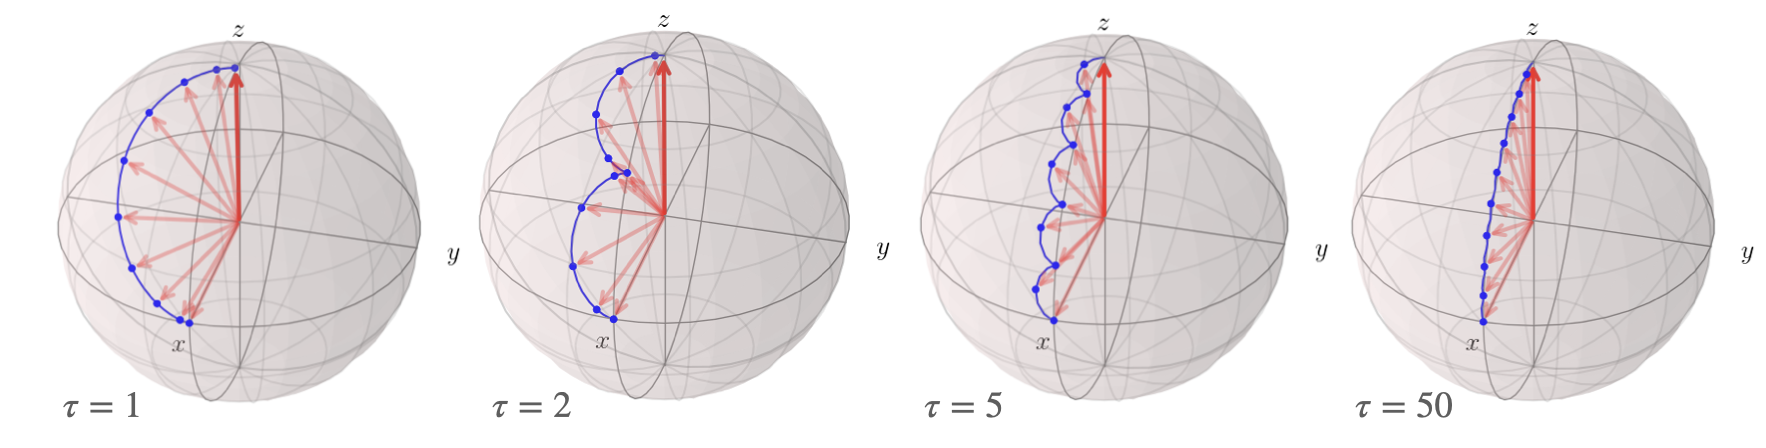
\includegraphics[width=0.9\linewidth]{images/magnetic_field_spin.png} \caption{Bloch sphere illustration of the single-spin system driven by the Hamiltonian of Eq.~\eqref{eq:rotating_spin_H} for different total driving times $\tau$.}\label{fig:bloch_rotating_spin}
    \end{figure}
    
    This specific example Let us first take a general case: for a dimensionless parameter $\lambda \in [0,1]$, let $H(\lambda)$ be a Hermitian operator that varies smoothly as a function of $\lambda$. This $\lambda$ may be the magnetic field orientation or any other parameter that can be varied in a quantum system. In fact, let's take $\lambda = \frac{t}{\tau}$, so that when $\tau \gg 1$, $H(\lambda)$ varies very slowly as a function of the time.  An initial quantum state $\ket{\psi(0)}$ evolves according to the Schr\"{o}dinger equation:
    \begin{equation}\label{eq:adiabatic_schrodinger}
        i\dv{\ket{\psi(\lambda)}}{\lambda} = \tau H(\lambda)\ket{\psi(\lambda)}
    \end{equation}
    
    \section{The adiabatic gauge potential}

    \section{Shortcuts to adiabaticity}
    
    Here I'm going to talk about Shortcuts to Adiabaticity (\hyperref[acr:sta]{STA})
    
    \subsection{Transitionless Driving}
    The form of the dynamical Hamiltonian enforcing this is \cite{berry_transitionless_2009}:
    \begin{equation}\label{eq:counterdiabatic}
        H_{\mathrm{CD}}(t) = H_0 (t) + i\hbar \sum_n (\ket{\partial_t n}\bra{n} - \bra{n}\ket{\partial_t n}\ket{n}\bra{n}),
    \end{equation}
    \subsection{Counterdiabatic driving}
    \subsection{Variational counterdiabatic driving}
    Following the methods of Ref.~\cite{sels_minimizing_2017}, the problem of finding the optimal adiabatic gauge potential can be cast as the minimisation of the Hilbert-Schmidt norm of the operators
    \begin{equation}\label{eq:Goperator}
     G_{\lambda}= \partial_{\lambda}H_\beta + i\comm{\mathcal{A}_\lambda}{H_\beta},
    \end{equation}
    which is equivalent to minimisation of the action
    \begin{equation}\label{eq:actionCD}
    \mathcal{S}(\mathcal{A}_{\lambda}) = \Trace{\left[G_{\lambda}(\mathcal{A}_{\lambda})^2\right]},
    \end{equation}
    with respect to $\mathcal{A}_{\lambda}$.
    \subsection{Nested commutator expansion}
    \subsection{Krylov methods}
